\documentclass[11pt]{article}
\usepackage[spanish]{babel}


%%%%%%%%%%%%%%%%%%%%%%%%%%%%%%%%%%
%%%%%%%%%%%%%%%%%%%%%%%%%%%%%   %%
%%        Datos Trabajo     %%  %%
%%%%%%%%%%%%%%%%%%%%%%%%%%%%%%%%%%
\newcommand{\titulo}[0]{Reto 5. Planeación financiera personal}
\newcommand{\materia}[0]{Finanzas Personales v1}


%%%%%%%%%%%%%%%%%%%%%%%%%%%%%%%%%%
%%%%%%%%%%%%%%%%%%%%%%%%%%%%%%%%%%
\usepackage{amssymb}
\usepackage{enumerate}
\usepackage{geometry}
\usepackage{mathtools}
\usepackage{multicol}
\usepackage{soul}

\usepackage{graphicx}
	\graphicspath{ {assets/} }

\usepackage{hyperref}
	\hypersetup{
			pdftex,
		        pdfauthor={bench},
		        pdftitle={...},
		        pdfsubject={...},
		        pdfkeywords={UVEG},
		        pdfproducer={Latex with hyperref, Ubuntu},
		        pdfcreator={pdflatex, or other tool},
			colorlinks=true,
				linkcolor=[rgb]{0,0,0.45},
				urlcolor=cyan,
				filecolor=green,
				citecolor=blue}

%%%%%%%%%%%%%%%%%%%%%%%%%%%%%%%%%%
%%%%%%%%%%%%%%%%%%%%%%%%%%%%%%%%%%

\title{\titulo}

\author{ Universidad Virtual del Estado de Guanajuato \textbf{UVEG} \\ 
\materia \\ Benjamín Rivera \\ 19015478 }
\date{\textit{Fecha de entrega:} \today}


%%%%%%%%%%%%%%%%%%%%%%%%%%%%%
%%        Documento         %%
%%%%%%%%%%%%%%%%%%%%%%%%%%%%%%%
\begin{document}
	\maketitle
	
	\begin{figure}[htp]
		\centering
		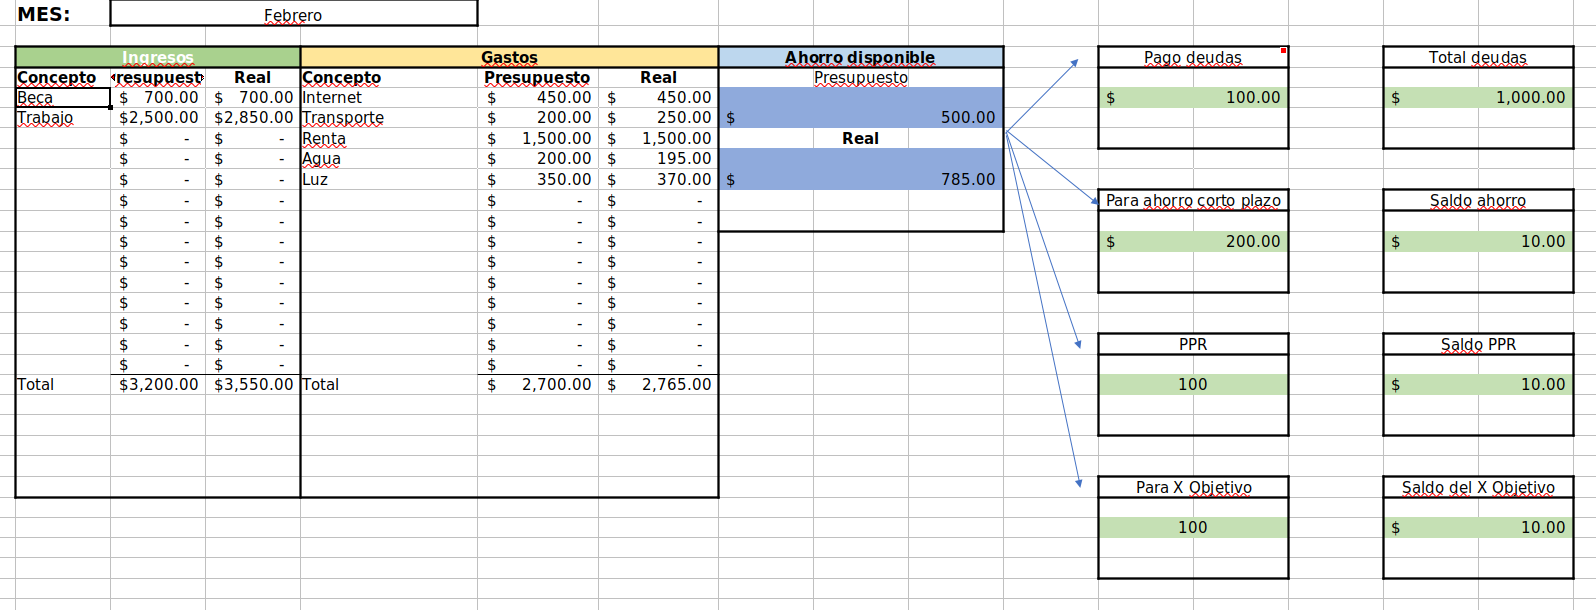
\includegraphics[width=1.1\textwidth]{assets/R5_U3.png}
		\caption{Presupueto muetra del mes de \textit{Febrero}.}
		\label{Capturas}
	\end{figure}
	
	\par Como este es una primera planeación de gastos, únicamente proporcionare la del primer mes, ya que no suponemos cualquier otro desperfecto o eventualidad y todas son idénticas (por ahora). Lo más fácil de notar al hacer esta actividad es que los ingresos (al menos en mi caso) son de las cosas más estables que habrá en el plan, las pequeñas variaciones dependen de las propinas que suelen dejar (aunque incluso esto se mantiene en un rango constante); mientras que por otro lado, los gastos son altamente variables, principalmente los servicios que se pagan por uso, además de que siempre puede haber imprevistos como una enfermedad, el aumento de algún producto o cualquier otro imprevisto que te pueda causar un gasto inesperado.
	
	\par Una vez que se nota todo lo que se muestra en esta planeación presupuestal, lo siguiente útil sería empezar a ajustar el plan en función con la realidad (porque esta varia constantemente con el tiempo) y con esto ir notando donde de pueden reducir gastos y, en caso de incluir nuevas fuentes de ingreso, ver cuales son las que dan un mayor beneficio. Como principal observación yo me la haría hacía mis gastos, el que sean la cosa más constante de mi planeación creo que debería ser algo importante a cambiar en esta situación; como alternativa inmediata para cambiar esto vería la creación de otra fuente de ingresos, aunque es algo que debo pensar con mayor detenimiento y evaluar las distintas opciones para ver cual es la que se ajusta mejor a mis tiempos, necesidades y capacidades.
	
	\par En general, tanto este trabajo como todos los que desarrolle en esta materia, me han permitido notar sutilezas en las que descuido mi salud financiera. Estos también me han presentado ciertas herramientas con las que ahora considero que podría mejorar la planeación de mi situación económica y, por tanto, también a mi salúd financiera. La mayoría de las cosas que note en este curso antes de este eran desconocidas para mi.

%%%%%%%%%%%%%%%%%%%%%%%%%%%%%%%%
%%         Bibliografia        %%
%%%%%%%%%%%%%%%%%%%%%%%%%%%%%%%%%%
	\begin{thebibliography}{X}
	
		\bibitem{1} Hoja de cálculo del presupuesto mensual personal. (s/f). Recuperado el 27 de enero de 2021, de \url{https://templates.office.com/es-es/hoja-de-cálculo-del-presupuesto-mensual-personal-tm16410113}
		
	\end{thebibliography}

\end{document}